\label{sec:policy_body}

The empirical results have a direct operational use: they
specify a decision rule for monitoring whether the post-ChatGPT
contraction is reaching the crowd-validated margin in a given
tag or portfolio.

\subsection{A value-calibrated early-warning system}
\label{ssec:pol_monitor}

A platform manager allocating scarce intervention effort
(contributor incentives, attribution mechanisms, moderation
attention) needs two things: a \emph{detection} signal for which
tags are losing high-value reusable flow, and a way to
\emph{size} the high-value consequence of a detected decline. We
build a tool that does both, and we let the data choose the
detection signal rather than assume our value index is it.

The decision has two margins. At the \emph{extensive} margin
(which tags to act on), a value-disproportionality \emph{ratio}
(VtD) is a poor detector---on the full 100-tag panel it ranks
realised 2025 high-value erosion at AUC $0.57$, far below the
activity-decline metric a platform already tracks (AUC $0.98$,
out of sample). This high AUC is not interpreted as an
independent behavioural prediction---its detection target contains
activity-derived high-value erosion---but as evidence that the
operational activity signal is sufficient for triage; the value of
calibration is evaluated separately by the budgeted-regret
experiment below. The practical conclusion is that platforms need
no bespoke value instrumentation to \emph{detect} where erosion is
largest: the system detects on activity. At the \emph{intensive}
margin (how much effort per selected tag), the value calibration
earns its place: allocating an intervention budget by the
value-calibrated high-value-at-risk (activity scaled by the
tag's high-value share) nearly attains the perfect-foresight
optimum (calibrated regret under $1\%$), whereas allocating by \emph{raw}
activity leaves regret of $3$--$5\%$ of the protectable
high-value flow (Table~\ref{tab:vtd_voi}, full panel,
out-of-sample on realised 2025 loss). The calibration thus has
positive, measurable value of information, even though it does
not---and need not---improve detection.

The artefact is therefore a \emph{value-calibrated} early-warning
system, not a value-detector. Its detection layer is the
activity signal (AUC $0.98$); its contribution is the
\emph{calibration} layer that converts an activity alert into the
decision-relevant quantity a manager lacks: for a flagged tag $t$,
$\widehat{\text{HV}}_t = (\text{activity deficit}_t)\times(\text{tag
high-value share})$, the activity signal scaled by the
value-margin gradient of \S\ref{ssec:results_value_weighted}; a
loss-derived threshold sets the alert cutoff from costs rather
than a mechanical mean. The value-disproportionality index
survives in a strictly secondary role---it describes \emph{what
kind} of decline a tag has (it is cross-sectionally orthogonal to
the activity level, $\rho=0.08$; Figure~\ref{fig:vtd_monitor}),
and that classification persists from 2024 onto the new 2025 data
($\rho=0.90$, $p<0.001$), so a manager can use it to choose
intervention \emph{type} (high-value-contributor retention for
value-disproportionate tags versus generic re-engagement for
proportional ones). The system is provided as a reproducible
script run on quantities a platform already records; it is
\emph{not} a deployed interface, and we run no manager user study.
A production dashboard and usability evaluation are future work
(\S\ref{sec:limitations}).

\begin{table}[ht]
\centering
\caption{Intensive-margin value of calibration, \textbf{full 100-tag 2025 panel} (out of sample). A manager allocates an intervention budget $B$ (a fraction of total tag activity) to protect realised 2025 high-value flow, ranking by efficiency. \textbf{Oracle} is the perfect-foresight cost-constrained optimum; \textbf{Calibrated} ranks by end-2024 high-value-at-risk; \textbf{Naive} by raw activity loss; \textbf{Random} averages shuffles. Cells are the share of realised 2025 high-value loss captured; the regret of a rule is $(\text{Oracle}-\text{rule})/\text{Oracle}$.}
\label{tab:vtd_voi}
\small
\begin{tabular}{lrrrrrr}
\toprule
$B$ & Oracle & Calibrated & Naive & Random & Regret$_{\text{calib}}$ & Regret$_{\text{naive}}$ \\
\midrule
10\% & 0.19 & 0.19 & 0.19 & 0.08 & 0.01 & 0.04 \\
25\% & 0.38 & 0.38 & 0.36 & 0.23 & 0.00 & 0.05 \\
40\% & 0.55 & 0.55 & 0.52 & 0.38 & 0.00 & 0.04 \\
50\% & 0.65 & 0.64 & 0.63 & 0.48 & 0.00 & 0.03 \\
\bottomrule
\end{tabular}
\end{table}

\begin{figure}[!htbp]
\centering
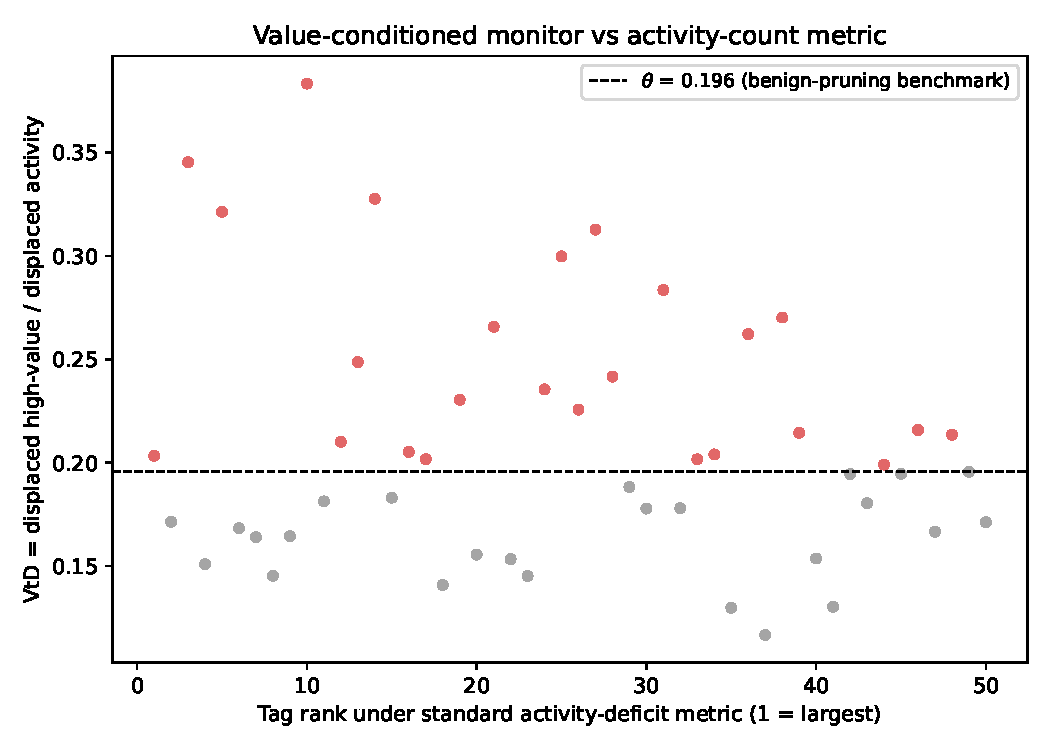
\includegraphics[width=0.78\textwidth]{figures/fig_vtd_monitor.pdf}
\caption{Value disproportionality versus the activity-count
metric. Each point is a tag, positioned by its activity-deficit
rank (horizontal) and VtD ratio (vertical); red points exceed the
benign-pruning benchmark $\theta=0.196$. The flat scatter
($\rho=0.08$) shows value disproportionality is close to
orthogonal to the \emph{size} of a tag's deficit. The activity
deficit remains the better predictor of erosion \emph{magnitude};
the monitor's contribution is the persistent disproportionality
dimension.}
\label{fig:vtd_monitor}
\end{figure}

\subsection{Implications for providers, managers, and
regulators}\label{ssec:pol_ai_providers}\label{ssec:pol_managers}\label{ssec:pol_regulators}\label{ssec:pol_welfare}

The asymmetry between activity and value is decision-relevant.
An AI provider or platform manager inferring training-corpus or
knowledge-production contraction from \emph{raw} post counts
overstates the funnel-qualified-post loss by a factor of roughly
$70{,}000/28{,}000\approx2.5$, because only about $40\%$ of raw
posts survive the support gates; and the value evidence
(\S\ref{ssec:results_value_weighted}) shows the displacement at
the crowd-validated tail is at least as strong relative to the
volume baseline. The dynamic concern that recursive training on
generated content degrades model quality
\citep{shumailov2024curse} gives providers a self-interested
reason to support attribution and contribution mechanisms (e.g.\
the May 2024 Stack Exchange--OpenAI agreement
\citep{stackexchange_openai_2024}). For regulators---e.g.\ the
training-data transparency provision of the EU AI Act
\citep{eu_ai_act_2024}---the sizing implication is that an
instrument framed on the LLM-substitutability margin should be
calibrated to the estimated channel ($\sim$5\% of the
trend-implied aggregate shortfall), not to the inferred
$65$--$71\%$ aggregate decline, which differs by an order of
magnitude. We do not estimate welfare and do not compare the
private productivity gains of LLM adoption against the public
shortfall: the two are in different units with different
horizons, and a static comparison would understate the dynamic
and distributional dimensions.

\subsection{What the magnitude does not
support}\label{ssec:pol_not_supported}

We do \emph{not} derive from the estimate: a welfare conclusion
(neither side of the trade-off is identified); an optimal-policy
recommendation (the social value of the marginal question is not
identified); an effect on innovation \emph{outcomes} (the DDD
estimates an innovation \emph{input}, not patents, products,
entry, or productivity); a generalisation beyond programming;
or a managerial intervention design (we do not identify the
elasticity of contribution to any specific instrument).
